\chapter{Simulationsumgebung}  
\label{ch:Simulationsumgebung}
Ohne eine angemessene Simulationsumgebung ist das ganze Projekt undenkbar. Nicht nur, dass das Training am realen Demonstrator schon wegen des Zeitaufwandes praktisch nicht möglich ist, auch die Konsistenz der Umgebung wage ich in Frage zu stellen.
Die Integration der vielen Rewards sind mit der Bildverarbeitung auch komplizierter und in einer Simulation zusätzlich präziser.
Da wegen vielen Gründen eine Simulation nötig ist und diese auch einen großen Teil der Arbeit ausgemacht hat, wird im folgenden Kapitel das Programm Unity vorgestellt. Außerdem wird unser Unity Projekt hinsichtlich der Implementierung und der Nutzung vorgestellt.

\section{Auswahl  der Umgebung}
\label{sect:Auswahl  der Umgebung}
Da bereits aus einer vorhergegangenen Arbeit und ein Projekt in Unity vorhanden war ist die Entscheidung hier sehr schnell gefallen.
Selbst ohne diesen Aspekt ist Unity aber eine gute Wahl. Neben einer Pythonschnittstellte, die für Reinforcemet Learning immer nützlich werden kann kann Unity auch noch mit einer großen Community und sehr guter Dokmentation punkten. Dadurch ist die Einarbeitungsphase relativ kurz und angenehm. Hinzu kommt noch die Toolbox ML-Agents. Diese stellt bereits Agenten zur verfügung, bei denen nur noch Hyperparameter gewählt werden müssen.  Eine schnelle, unkomplizierte Möglichkeit mit dem Training zu beginnen.

\section{Unity}
\label{sect:Unity}
Unity ist eine von Unity Technologies entwickelte multiplattform Entwicklungsumgebung zum Erstellen von Videospielen. Unsere Anwendungist zwar kein Videospiel im herkömmlichne Sinn, aber von der Physikengine können wir trotzdem gebrauch machen. Neben dreidimensionalen Umgebungen bietet Unity auch einen 2D-Modus an, der für unsere Anwendung ausreichend ist. Die Programmiersprache unserer Wahl ist c\#, jedoch ist es auch möglich in UnityScript und Boo benutzerdefiniertes Verhalten zu programmieren.\\
Wir haben die Unity Version 2020.1.6f1 genutzt.\\
Die Version des ML-Agents Toolkits, die zum Einsatz kam, lautet 2.1.0-exp.1

\subsection{Kurze Einführung}
\label{subsect:Kurze Einführung}

Die kurze Einführung in Unity soll anhand des User Interfaces geschehen. Diese ist keineswegs vollständig und soll auch nur ein grobes Verständnis für Fachfremde ermöglichen. Die Markierungen im Bild \ref{untiy_interface} werden im Folgenden erklärt.

\begin{figure}
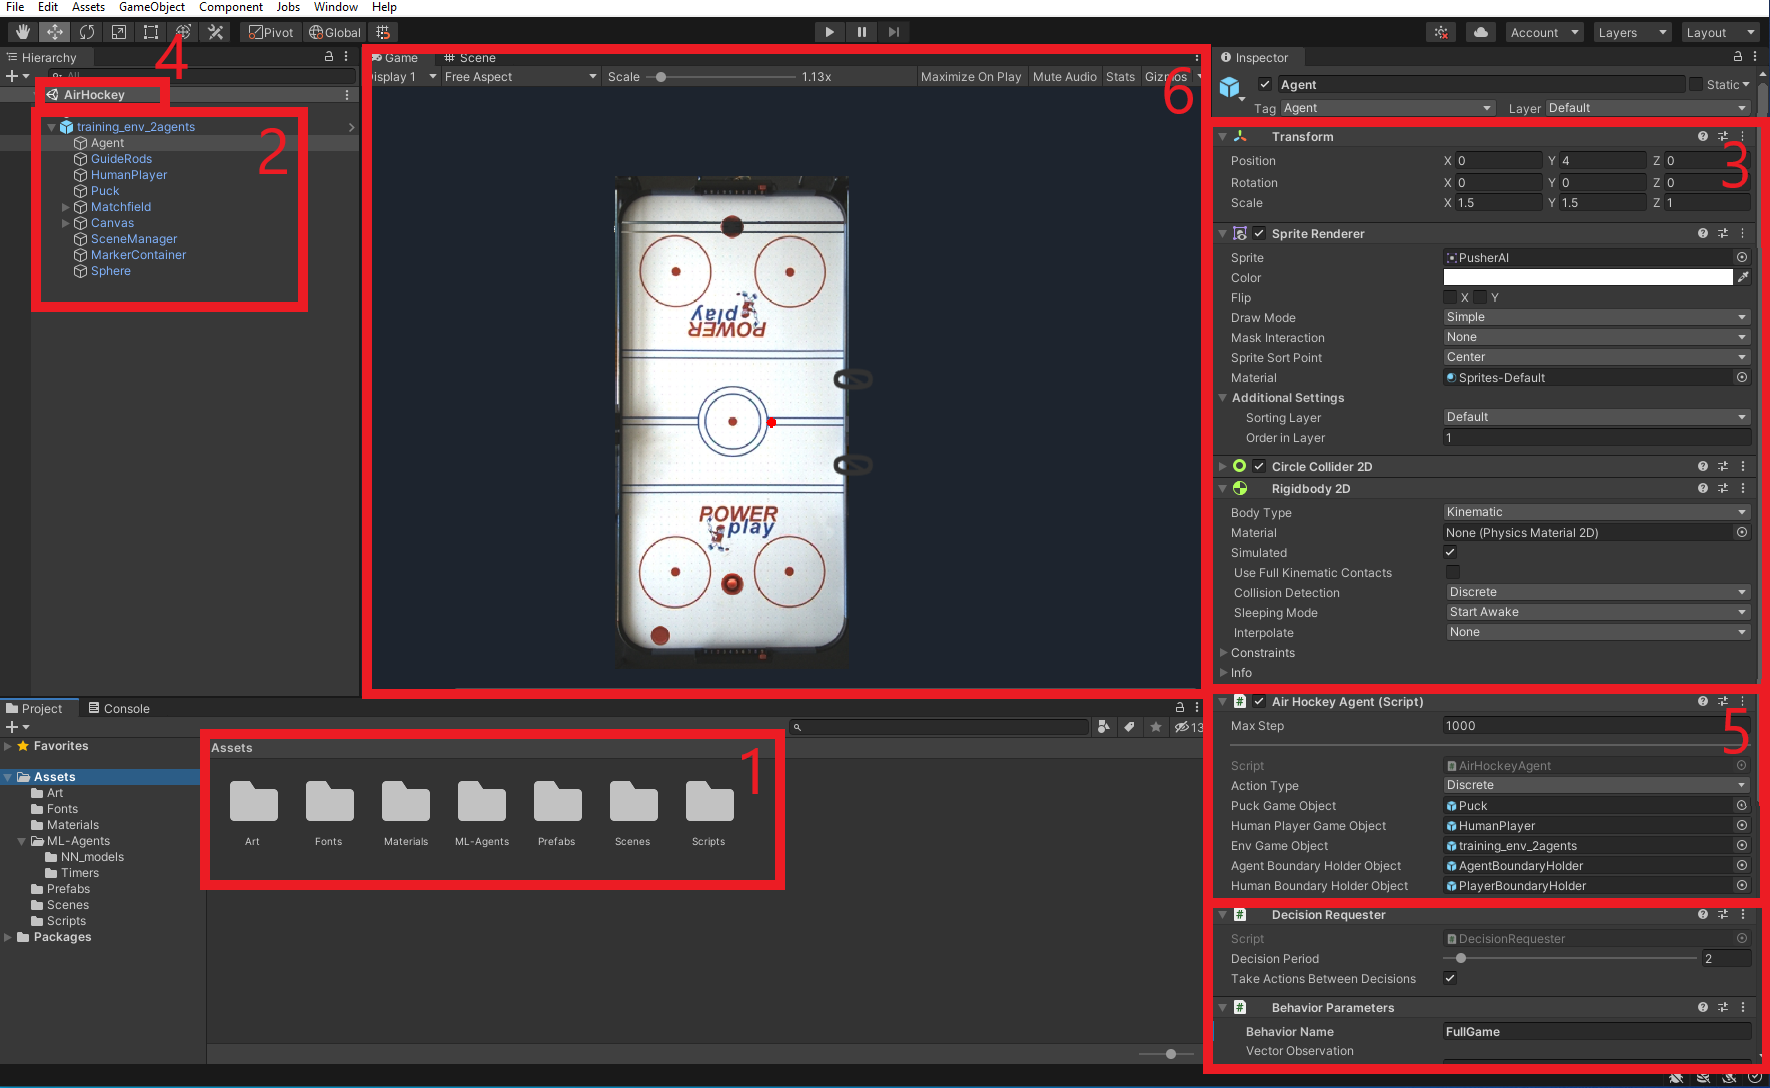
\includegraphics[scale=0.3]{images/unity_interface_marked}
\label{unity_interface_pic}
\caption{Benutzeroberfläche von Unity mit Markierungen}
\end{figure}

\begin{itemize}
\item \underline{Assets (1)} \\
Assets beinhaltet diverses. Neben Grafiken, vorgefertigten Materialien und Szenen sind hier auch die Skripte zu finden

\item \underline{GameObjects (2)} \\
GameObjects sind das zenrale Konzept von Unity. Jedes Objekt, jede Kamera und jede Grafik ist durch ein Gameobject definiert. Die Funktionalitäten eines GameObjects werden durch die Components hinzugefügt. Die GameObjects sind in einem Hierariebaum in der Scene  eingeordnet.

\item \underline{Components (3)} \\
Components geben den GameObjects ihre Funktionalität. Ein GameObject kann mehrere Components haben. Beispiele für Components sind Transform (zuständig für die Position), Collider(zuständig für die Interaktion in der Physiksimulation) und auch Skript.

\item \underline{Scene (4)} \\
Eine Scene (Szene) besteht aus GameObjects. Es ist im Prinzip die Wurzel des Hierarachiebaums. Zur Spieleentwicklung könnten hier unterschiedliche Level als underschiedliche Scenes interpretiert werden. In unserem Fall sind nur zwei Scenen vorhanden: eine mit einem Spielfeld zum selbst spielen und testen und eine mit acht Feldern zum beschleunigten Training.

\item \underline{Script (5)} :\\
Scripts sind auch Components. Sie sind die Möglichkeit selbst Verhalten zu definieren. Es kann sich in Scripts auf GameObjects bezogen werden. Mit ihrer Hilfe können Parameter wie Material oder Position geändert werden. Objekte können auch entfernt oder eingefügt werden.

\item \underline{Visualisation (6)} :\\
In diesem Bereich kann sowohl das Bild einer Kamera, und  damit die Ansicht im Spiel, beobachtet werden als auch eine Darstellung aller GameObjects in der Scene. Objekte können hier auch verschoben oder gedreht werden.
\end{itemize}

\subsection{Airhockey Projekt}
\label{subsect:Airhockey Projekt}

In diesem Unterkapitel werden die einzelnen GameObjects und die wichtigstens Components im Projekt vorgestellt und erklärt. Ziel ist es dabei nicht auf jedes Detail einzugehen, sondern die Arbeit für Folgeprojekte zu erleichtern. Rein optische Aspekte, wie zum Beispiel die Anzeige des Spielstandes, werden nicht betrachtet. Außerdem wird nur auf die Scene mit einem Feld eingegangen,  dann die Anpassungen, die zum Kopieren gemacht werden müssen sind nicht maßgeblich. Die folgenden GameObjects sind auch in der Abbildung \ref{unity_interface_pic} zu finden.\\

\underline{Agent} :

\begin{figure} [h]

\begin{minipage}[t]{0.6\textwidth}
\vspace{0pt}
Das Agent ist eines der zentralen GameObjects. Es hat eine Sprite Renderer Component. Dadurch kann es mit einer .png Datei Visuallisiert werden. Der Agent ist also ein Objekt, dass im Spiel zu sehen ist. Auf der rechten Seite ist zu sehen, wie es im Projekt zu sehen ist.
\end{minipage}
\hspace{0.1\textwidth}
\begin{minipage}[t]{0.2\textwidth}
\vspace{0pt}
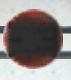
\includegraphics[width=\textwidth]{images/agent_unity}
 \caption{Ansicht des Agenten in Unity}
 \label{unity_agent}
\end{minipage}
\end{figure}

Das Agent GameObject enthält auch eine Circle Colider Component. Mit der Rigidbody Component zusammen wird die Phsyik(Reibung, Bewegung, Kollision) simuliert.\\
Ein weiterer Component des Agent Objekts ist das Script Airhockey Agent. Die Funktion von diesem Script ist die Interaktion mit der ML Agents Toolbox. Es werden sowohl in die anfalleden Rewards entsprechend des Spielverlaufes an das  Netzwerk zurück gegeben, als auch die Actions entgegen genommen und damit die Umgebung (Bewegung des Agenten) beeinflusst. Zu Episodenbeginn werden in diesem Script auch die Positionen von Agent und Spieler (Pusher) zurück gesetzt. \\
Des weiteren beinhaltet das Agent GameObject auch noch eine Decission Requester Componente. Mit ihrer Hilfe wird regelmäßig, entsprechend des Parameters Decision Periode, eine Action vom Netzwerk angefordert. Die Behavior Parameter Componente ist, neben Decison Requester, zur Parametrisierung der Nutzung des ML Agents Toolkits nötig. Hier kann die Dimension sowohl des Actionspaces als auch die der  Obseration festgelegt werden. Auch Angaben zur Interferenz können hier gemacht werden. \\


\underline{HumanPlayer} :

\begin{figure} [h]

\begin{minipage}[t]{0.6\textwidth}
\vspace{0pt}
HumanPlayer ist das GameObject des zweiten Spielers. Es hat auch eine Sprite Renderer Component. Die Visualisierung ist rechts zu sehen. Da diese Objekt auch am Spiel teilnimmt hat es auch die Components Circle Collider und Rigidbody.
\end{minipage}
\hspace{0.1\textwidth}
\begin{minipage}[t]{0.2\textwidth}
\vspace{0pt}
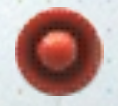
\includegraphics[width=\textwidth]{images/pusher_unity}
 \caption{Ansicht des Pushers in Unity}
 \label{unity_pusher}
\end{minipage}
\end{figure}

HumanPlayer hat auch die Components Decission Requester und Behavior Parameters. Damit wird das Selfplay ermöglicht. In unserer Implemetierung wird die Verion des Agenten, die den HumanPlayer bewegt nicht trainiert. Das ML Agents Toolkit wird hier nur zur Interferenz genutzt. \\
Das Objekt enthält auch ein Script. Im Gegensatz zum Airhockey Agents Script werden hier aber eine Rewards zurück gegeben sondern nur die Observations und die Actions behandelt. Das reicht auch aus, denn dieser Agent soll ja garnicht ständig mittrainieren, sondern nur das Selfplay ermöglichen. Wenn er zu schwach wird, wird einfach die stärkere Version vom Agent übertragen. Im Script ist auch die Option den HumanPlayer selbst zu steuern implementiert. Entweder mit der Tastatur oder mit einem Controller kann so der Agent herrausgefordert werden. \\

\underline{Puck} :

\begin{figure} [h]

\begin{minipage}[t]{0.6\textwidth}
\vspace{0pt}
Der Puck ist auch ein Objekt, dass wie der HumanPlayer und der Agent am Spiel teilnehmen. Deshalb hat es auch die Components Circle Collide und Rigidbody.  Die Components, die für das ML Agents Toolkit nötig sind, sind hier aber nicht nötig. Trotzdem gibt es auch hier ein c\# Script, dass das Verhalten des Pucks bestimmt.
\end{minipage}
\hspace{0.1\textwidth}
\begin{minipage}[t]{0.2\textwidth}
\vspace{0pt}

\includegraphics[width=\textwidth]{images/puck_unity}
 \caption{Ansicht des Pucks in Unity}
 \label{unity_puck}
\end{minipage}
\end{figure}
Abhänig vom Spielszenario wird in diesem Script die Startposition und die Startgeschwindigkeit des Pucks festgelgt. Auch der Spielstand wird hier mitgezählt. Die Circle Collider Componente  des Pucks erlaubt es ein Event bei Kollision mit anderen Objekten auszulösen. Wenn der Spielfeldrand am Tor des  Agenten getroffe wird, kann das mit Hilfe eines GameObjects ohne Renderer erkannt werden. Es kann mit einer Box Collider Componente ein Event ausgelöst werden, das den Spielstand anpasst. Das gleiche System wird auch auf der anderen Seite angewendet. \\

\underline{Matchfield} :

\begin{figure} [h]

\begin{minipage}[t]{0.6\textwidth}
\vspace{0pt}
Das GameObject Matchfield hat selbst nur eine Sprite Renderer Component, die ein Bild des Airhockeytisches zeigt. Jedoch sind diesem Objekt hierarchisch weitere untergeordnet. Diese untergeordneten Objekte sind aber alle ohne Renderer Component und deshalb in der Spielansicht unsichtbar. Sie sind nur wegen ihrer Position interessant. Sie dienen um das Spielfeld in Zonen einzuteilen. Die zulässigen Positionen von Agent, HumanPlayer und Puck werden damit auf das Spielfeld oder die jeweilige Hälfte limitiert. Die GameObjekts, die zum Tore zählen genutzt werden sind auch Childobjekte (hierarchisch untergeordnete Objekte) des Matchfieldes.
\end{minipage}
\hspace{0.1\textwidth}
\begin{minipage}[t]{0.2\textwidth}
\vspace{0pt}
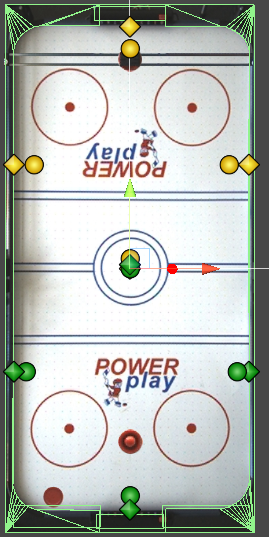
\includegraphics[width=\textwidth]{images/matchfield}
 \caption{Spielfeldbegrenzungen in Unity}
 \label{unity_matchfield}
\end{minipage}
\end{figure}
Das Matchfield hat kein Script, es wird sich nur von anderen Scripts auf die GameObjects von Matchfield bezogen. Die Transform Component, die die Position eines Objects angibt, wird dabei ausgelesen. Mit vier Objekten lässt sich damit ein rechteckiger Bereich festlegen. \\

\underline{training\_env\_2agents} :\\
Diesem Objekt sind, abgesehen von der Kamera, alle anderen GameObjects untergeordnet. Es dient als Container für das ganze Spiel. Das Objekt dient hauptsächlich zwei Zecken:
\begin{itemize}
\item Das ganze Spielfeld kann einfacher kopiert und verschoben werden. Die Positionen der Childobjekte bleiben beim Verschieben des übergeordneten Objekts relativ zu diesem unverändert. Felder könne dadurch schnell über und nebeneinander kopiert werden.
\item Das envScript ist in diesem GameObject ein Component. In diesem Script werden alle Rewards festgelegt. Auch der Spielmodus wird hier ausgewählt. Näheres zu den Rewards und den Spielmodi wir im Kapitel \ref{subsect:Airhockey Projekt} erläutert.
\end{itemize}